\documentclass[a4paper, 11pt]{report}

\usepackage{color}
\usepackage[utf8]{inputenc}
\usepackage[frenchb]{babel}
\usepackage{graphicx}
\usepackage{epstopdf}
\usepackage{listings} 
%\usepackage[cm]{fullpage}
\usepackage[a4paper]{geometry}

\graphicspath{{./img/}}

\def\maketitle{
  \hspace{-2cm}
    \hbox to 0px{
\includegraphics[scale = 0.7]{LOGO_UNS.png}}  
    \hbox to 12cm{}  
    \hbox to 0px{
\includegraphics[scale = 1.1]{Polytech.jpg}} 
  \vfill
  \begin{center}\leavevmode
    \normalfont
    ~~\\
    ~~\\
    ~~\\
    ~~\\
    ~~\\
    ~~\\
    ~~\\
    ~~\\
    ~~\\
    ~~\\
    ~~\\
    {\LARGE \textbf{Algorithmique géométrique\\Recherche des voisins}\par}%
    ~~\\
    ~~\\
    {\Large Auteurs:\textbf{Romaric~Pighetti et Clément~Léger} \par}%
    ~~\\
    ~~\\
    {\Large Encadrant: \textbf{Mr Devillers} \par}%
    ~~\\
    ~~\\
    {\Large \'Ecole: \textbf{Polytech'Nice-Sophia} \par}%
    ~~\\
    ~~\\
    {\Large \textbf{\today}   \par}%
    ~~\\
    ~~\\
    \end{center}
  \vfill
  \null
  \clearpage
}

\begin{document}
	\addtolength{\voffset}{-2cm}
	\addtolength{\textheight}{5cm} 

  \maketitle
  
  \section*{Introduction}
  Le but de ce projet est de trouver, dans un ensemble de points coloriés du plan, le point le plus proche 
  d'un point requête ayant une couleur donnée. Ceci en énumérant dans l'ordre croissant de leur distance à la 
  requête tous les points parcourus avant d'avoir trouvé le point recherché. La Figure~\ref{exemple} montre 
  le résultat d'une exécution de l'algorithme.
  
  	\begin{figure}[!h]
	\begin{center}
	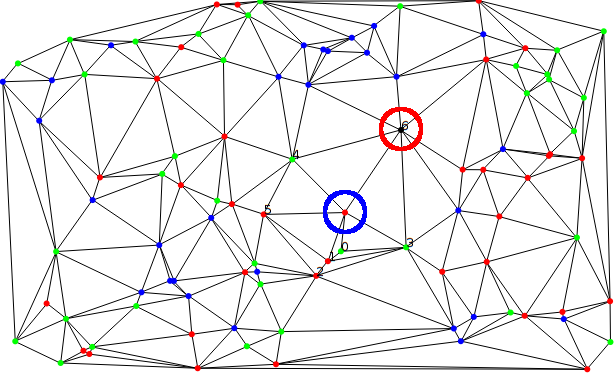
\includegraphics[width=400px]{screen.png}
	\end{center}
	\caption[]{Image d'origine}
	\label{exemple}
	\end{figure}
	
  \section*{Algorithme}
  La procédure générale de l'algorithme est la suivante:
  \begin{enumerate}
  \item Une requête (q,c), q étant un point et c une couleur, est passée par l'utilisateur à l'lgorithme. 
  On initialise le compteur n à 0, n nous permettra de numéroter nos points. 
  \item Il insert ensuite les voisins de q dans la triangulation dans un arbre binaire de recherche (ABR) qui trie
  ces points dans l'ordre de leur distance à q, le plus petit étant la racine. 
  \item L'algorithme récupère alors p, la racine de l'arbre. On lui donne le numéro n, on incrémente n. 
  \item Si la couleur de p est c ou que l'on a parcouru tous les points, on s'arrête. 
  \item Sinon, on insère les voisins de p que l'on avait pas déjà insérés et qui sont 
  différents de q dans l'ABR et on reprend à partir de l'étape 4.
  \end{enumerate}
  Les Figures~\ref{algo} et \ref{find} donne avec plus de détail le fonctionnement de ce dernier, notament 
  dans les cas limites où l'on se trouve au bord de la triangulation et que l'on ne veut pas insérer les points 
  infinis.

  	\begin{figure}[!h]
	\begin{center}
	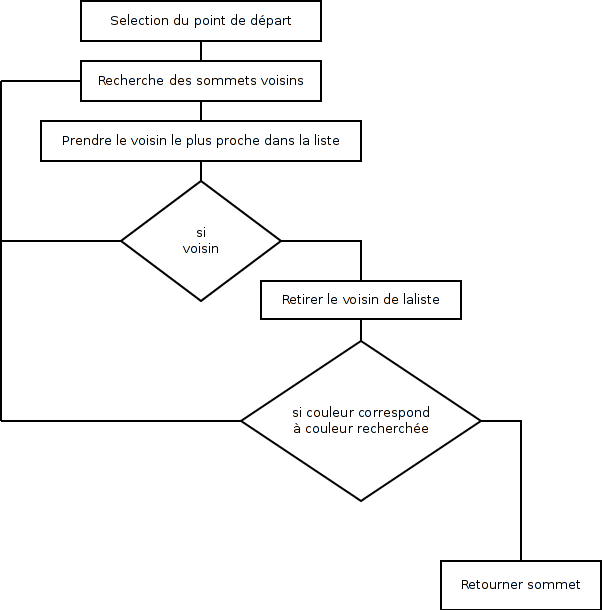
\includegraphics[height=400px]{algo.png}
	\end{center}
	\caption[]{Algorithme}
	\label{algo}
	\end{figure}

  	\begin{figure}[!h]
	\begin{center}
	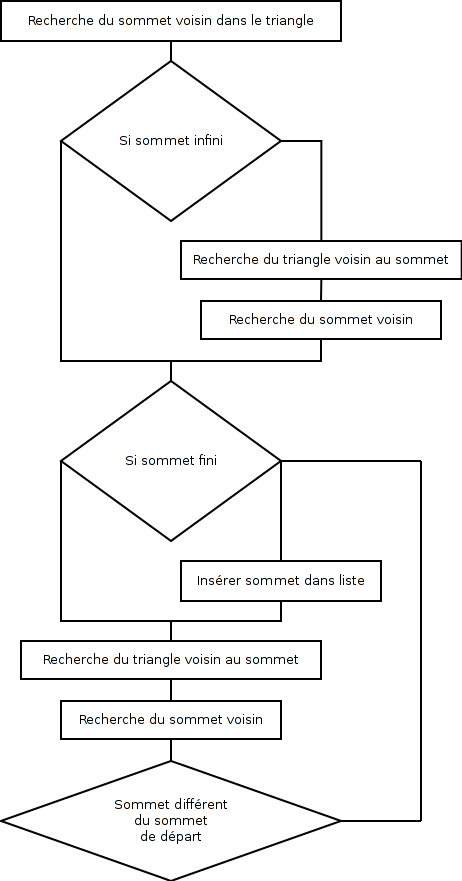
\includegraphics[height=400px]{findNeighborVertices.png}
	\end{center}
	\caption[]{find neighbours vertices}
	\label{find}
	\end{figure}

  \section*{Complexité}
  La complexité dépend du nombre de points parcourus avant d'atteindre le point de la couleur recherchée.
  Si on appelle k le nombre de points parcourus, on a alors les données suivantes:
  \begin{itemize}
  \item La complexité de l'insertion dans un ABR est en log du nombre d'éléments présents dans l'arbre.
  \item La complexité de la suppression de la racine est aussi en log du nombre d'éléments.
  \item Le nombre de voisins moyens d'un point dans la triangulation est 6.
  \item On aura donc en général 5 insertions et une suppression à faire par boucle.
  \end{itemize}
  Notre complexité est approximativement égale à $\sum_{i=1}^{6 k} (i * log(i) ))$ (On ne prend pas en 
  compte les suppressions, on fait comme si l'on avait seulement des insertions mais celà ne changera pas 
  l'ordre de grandeur).\\
  Or, $\forall i, log(i) < log(k)$, on a donc\\
  $\sum_{i=1}^{6 k} (i * log(i) )) <  log(k) * \sum_{i=1}^{6 k} (i)) = \frac{6 k * (6 k + 1) }{ 2 * log(k)} \\
  \Rightarrow \sum_{i=1}^{6 k} (i * log(i) )) = O(k^2 log(k))$\\
  On a donc une complexité en $O(k^2*log(k))$ avec k le nombre de points parcourus.\\
  Le nombre de points parcourus en moyenne avant d'atteindre la couleur recherchée dépend ensuite de la
  statistique de répartition des couleurs entre les points.

  \section*{Difficultés rencontrées}
  La prise en main et la modification de l'interface graphique réalisée à l'aide de Qt a été un premier défi. Une
  fois cette opération effectuée, le plsu difficile a été la recherche des fonctions nécessaires à l'algorithme 
  dans la documentation de CGAL. L'algorithme en lui même étant relativement simple il ne nous a pas posé 
  de problème.

  \section*{Conclusion} 
  Dans le cas où la triangulation de Delaunay est fournie, cet algorithme est en moyenne plus efficace qu'un 
  algorithme classique dans lequel on trierai l'ensemble des points. En revanche, si l'on doit construire la 
  triangulation, cette construction a une complexité de $n log(n)$, ce qui est la complexité du tri de 
  l'ensemble des points, cet algorithme devient alors beaucoup moins efficace. En revance, il peut être 
  intréressant de l'utiliser tout de même dans le cas où l'on a plusieurs recherches à faire sur le même 
  ensemble de points.

\end{document}
